\section{Theory}

The basic principle of an oscillator is to generate a continuous and periodic AC signal of desired frequencies. In its implementation, it is basically an amplifier circuit with positive feedback.

\subsection*{Working principle}

Let's say some input sinusoidal signal is applied to the input. At the output, the input signal will get multiplied by the gain of this amplifier, $V_o = AV_i$. Now, this output signal is given as an input to the feedback circuit. The feedback circuit is typically a frequency selector or resonant circuit. Let $\beta$ be the fraction of $V_o$ that is feedback as input into the system, i.e. $V_f = \beta V_o$. Now the input voltage is removed from the circuit. After removing $V_i$, whether we will get sustained oscillations or not depends on the product $A\beta$, which is known as the \textbf{loop gain} of the oscillator.

\begin{figure}[H]
    \centering
    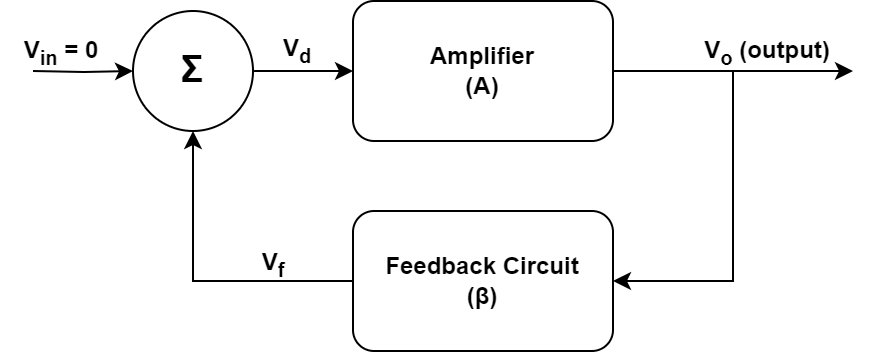
\includegraphics[width=0.85\columnwidth]{images/block.png}
    \caption{Block diagram for a typical oscillator circuit}
    \label{block}
\end{figure}

If $A\beta<1$, the oscillator exhibits a decaying oscillation and the signal eventually decays to zero. If $A\beta>1$, the output oscillation grows and becomes unbounded, eventually railing out the system. In other words, only when $A\beta=1$ and when the phase difference is an integral multiple of $360^{\circ}$ will the oscillator show stable oscillation.

These conditions are summarized in \textbf{Barkhausen's Criteria} for sustained oscillation,

\begin{enumerate}
    \item The magnitude of the loop gain should be equal to 1, i.e. $A\beta=1$
    \item Phase Shift introduced by the amplifier and the feedback circuit should be 0 or $360^{\circ}$.\\
\end{enumerate}

Without any input voltage, electronic oscillators use thermal noise to produce oscillations. When the circuit is turned on, all frequency components of the noise get amplified, which is given as the input to the feedback circuit. Since the feedback circuit is a frequency-selective circuit, only one particular frequency whose phase shift is 0 will get added back to the input. Hence, the noise signal of a desired frequency will show sustained oscillation.\\

\noindent From the block diagram (Fig. \ref{block}), 

\begin{align}
    V_o &= A(V_f + V_i) \nonumber\\
    &=A(\beta V_o) + AV_i \nonumber\\
    \implies AV_i &= V_o(1-A\beta) \nonumber\\
    \implies \frac{V_o}{V_i} &= \frac{A}{1-A\beta}
\end{align}

Since $V_i=0$, $\frac{V_o}{V_i}=\infty$. This means that on the right-hand side, $1-A\beta=0$, or $A\beta=1$, which is the Barkhausen condition. 

\subsection*{RC Phase Shift Oscillator}

RC phase shift oscillators produce stable sine waves and are used for low-frequency signal generation (typically in the range of audio frequencies).

Here, we use the op-amp as the amplifier and 3 cascaded networks as the frequency-selective feedback circuit. Since the op-amp is used in inverting mode, there is a $180^{\circ}$ phase shift. So, to generate sustained oscillations, the additional $180^{\circ}$ phase shift is achieved by the RC network.

Phase shift produced by a single RC stage is given by,

\begin{align}
    \phi = \taninv{\frac{X_C}{R}}
\end{align}

When $R=0$, $\phi=90^{\circ}$. Thus by cascading two RC stages, we can achieve $180^{\circ}$ phase shift. But practically since this requires $R$ to be 0, it means there is no gain. Hence, practically we use 3 RC stages each with a phase shift of $60^{\circ}$.

\begin{figure}[H]
    \centering
    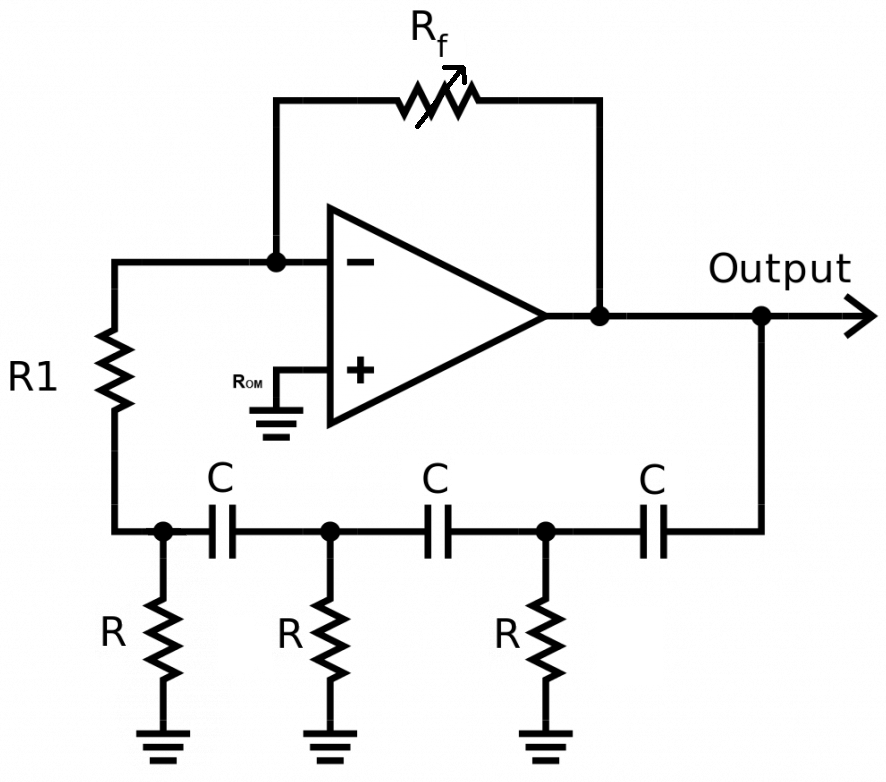
\includegraphics[width=0.7\columnwidth]{images/circuit2.png}
    \caption{Circuit diagram for the experimental setup}
    \label{circuit}
\end{figure}

The frequency of oscillation of the RC network is given by,

\begin{align}
    f = \frac{1}{2 \pi \sqrt{2N} RC} = \frac{1}{2\pi\sqrt{6}RC}\,\,\,[\because N=3] \label{freq}
\end{align}

Similarly, one can derive the gain of the RC network to be $\beta = 1/29$. Therefore to fulfill the Barkhausen criteria, we require the op-amp gain to be at least 29. Or,

\begin{align}
    \bigg|\frac{R_f}{R_1}\bigg| = 29 
\end{align}

One can also use \textbf{Lisssajous curves} to study the behavior of oscillator circuits. Lisssajous curves describe the family of curves which are formed by the superposition of two perpendicular oscillations in x and y directions of different angular frequencies. By using a secondary sinusoidal input source (a function generator) with variable frequency, we can observe these curves (using the X-Y mode of the oscilloscope).

These patterns form closed shapes if the frequencies are whole number ratios, i.e. at certain harmonics. 
% ======================================================================================
\section{Apparatus}

\begin{enumerate}
    \item OPAMP 741 Chip
    \item Resistors
    \item Oscilloscope
    \item DC Power Supply
    \item Function Generator
    \item Potentiometer
    \item Breadboard
    \item Connecting Wires
    \item Multimeters
\end{enumerate}